	
	After finding the optimal number of particles, we aimed for finding an adequate number of beams for the sensor reading towards an accurate and fast implementation.
	
	On the simulation, we let the robot localise itself into the first map and we measured the convergence time of the particle filter and the distance error relative to the actual robot's position, we vary the number of beams from 5 to 40 using increments by 5 and running each experiment 500 times. 
	
	We present the results on (Figure \ref{fig:NumBeams}) and we  inferred that more sensor beams leads to a more accurate pose's estimation but also increases the computational time for convergence since more operations are required. Thus, we select 10 beams as an adequate value since offers both accuracy (mean error of 1.44cm) and fast computation time ( mean 3.34 seconds for convergence). Thus we use 10 beams for further experiments and implementation. 
	
	
	\begin{figure}[h]
    \centering
		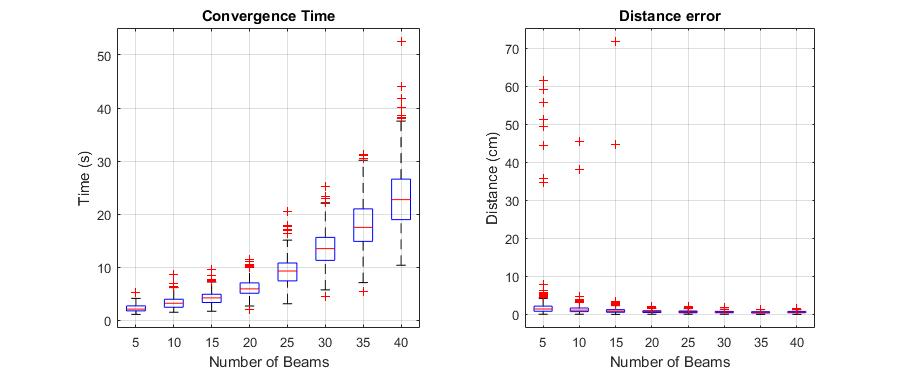
\includegraphics[width=.75\textwidth]{NumberOfBeams}
      \caption{Selecting an adequate number of sensor beams}
    \label{fig:NumBeams}
 	\end{figure}
	

	 
\FloatBarrier
	
	